%!TEX root = ../dissertation.tex
\begin{savequote}[75mm]
There is nothing sharp in nature.
\qauthor{Dr. Julian L\'eonard}
\end{savequote}
%Wie kommt es \textinterrobang

\chapter{Critical behavior of the \newline many-body-localization transition}
\label{sec:ch6}

We have, up till now, described quantum thermalization and MBL in terms of their resultant dynamical behavior from the integrability, or lack there of, of the quantum system. This behavior if a consequence of a qualitative change of the properties of the eigenstates at a finite disorder value where the two phases, thermalizing and many-body localized, have been theoretically predicted in the extreme value cases for short-range interacting systems in one-dimension \cite{Pal2010,Basko2006,Huse2013,Nandkishore2015,Imbrie2016,DAlessio2016}. This type of non-equilibrium phase transition is often referred to as an eigenstate phase transition since the properties of the individual excited eigenstates themselves change qualitatively at a finite value\cite{Pal2010,Huse2013}. However, understanding the exact transition behavior requires the the ability to exactly diagonalize the entire Hamiltonian since it relies on access to these highly excited eigenstates.\footnote{There are many theoretical proposals for this critical behavior that do not use exact diagonalization, but the validity of their results is unknown without either comparison to exact diagonalization or experimental results.} Such numerical approaches, while exact, are limited to relatively small finite sizes based upon the exponential growth of Hilbert space dimensionality with physical size\cite{Setiawan2017,Khemani2017}. Other numerical approaches, such as renormalization group theories (RG)\cite{Potter2015,Vosk2015,Zhang2018} work on significantly larger sizes but are implemented via a self-consistent set of rules that may not accurately capture the critical behavior due to the expected large, non-local entanglement at the critical point\cite{Alet2018,Abanin2018}. These same set of limitations do not restrict our experimental realization of an MBL system and in principle can faithfully perform exact simulations of the correct behavior for large systems. Although, a new practical limit emerges experimentally based on coherent evolution time. The practical limit of measuring out successive decades of time evolution require exponentially more experimental runs to overcome the increased post-selection rates.\footnote{Additional estimates of evolution time can be made from using the spontaneous scattering rate measurements in \S \ref{sec:ch2_heating}.} All results in this chapter will derive from time evolution up till $t\approx100\tau$.

While both non-equilibrium phases are well understood theoretically and can be successfully described by phenomenological models\cite{Serbyn2013b,Huse2014,Nandkishore2015}, the transition between these two phases remains an open question\cite{Grover2014,Vosk2015,Potter2015,Khemani2017,Alet2018,Abanin2018,Zhang2018}. Several experiments have probed slow transport properties through local observables near this critical regime\cite{Luschen2017,Bordia2017}. While such anomalous transport has been predicted theoretically\cite{Agarwal2015,Setiawan2017,Zhang2018}, identifying anomalous transport as quantum critical dynamics is experimentally challenging, since similar behavior can also originate from stochastic effects: inhomogeneities in the initial state\cite{Luitz2016} or the coupling to a classical bath \cite{Nandkishore2014,Luschen2017b}. We overcome these challenges in our experiment with our protocol by evolving a pure, homogenous initial state under unitary dynamics where we additionally utilize post-selection to exclude coupling to the environment by atom loss\cite{Luschen2017b,Lukin2019}. In this chapter, I present our results in this critical regime where we observe system-size dependent thermalization, anomalous transport, and correlations that span the entire system and persist up to high orders near the critical point\cite{Rispoli2018}. We additionally observe behavior in support of a proposed microscopic mechanism that leads systems at intermediate disorder strengths critically towards thermalization via a sparse resonant network\cite{Potter2015,Khemani2017,Rispoli2018,Herviou2019}. 
%\cite{Grover2014}
%\cite{Khemani2017,Khemani2017a,Setiawan2017}
%\cite{Vosk2015,Potter2015}


\section{Critical behavior and phase transitions}

Quantum phases are described by their local order parameter and their transition from one order to another, in any physical system, happens smoothly. This smooth cross over is typically limited by either the system size or temperature of the system. This regime of the smooth cross over tends to sharpen (shrink) as the system is either cooled to lower temperatures or the system size is increased. This shrinking of the smooth crossover demonstrates that the system was only critically limited by an external property; it will approach a particular phase in the $T=0$ or infinite-size limit. This smoothness has to do with the relationship of the finite correlation length at the transition as compared to the system size or the temperature to the minimum gap in the system. The scaling behavior of these transitions are dependent upon only global properties such as dimensionality and internal symmetries -- making the theory describing this critical behavior universal: it applies across a wide variety of physically different transitions as long as they have these same global properties \cite{Sachdev2011}. 

\subsection{Critical dynamics in equilibrium phase transitions}

The dynamics at non-equilibrium phase transitions are inherently different from those associated with critical behavior at equilibrium phase transitions.\footnote{However, one might consider that all phase transitions are eigenstate transitions and equilibrium quantum phase transitions focus only on the lowest energy eigenstate -- the ground state.} A traditional approach for the theory of ground state phase transitions has seen wide success in describing phase transitions within a set of universal classes with qualitative distinctions only changed by symmetries, interaction range, and dimensionality of the system. Therefore, it is natural to try and understand which, if any, of these traditional concepts may apply to non-equilibrium phase transitions and their critical behavior. In the following sections, the behavior associated with criticality in a traditional equilibrium quantum phase transition is discussed.

\begin{figure}[t!]
		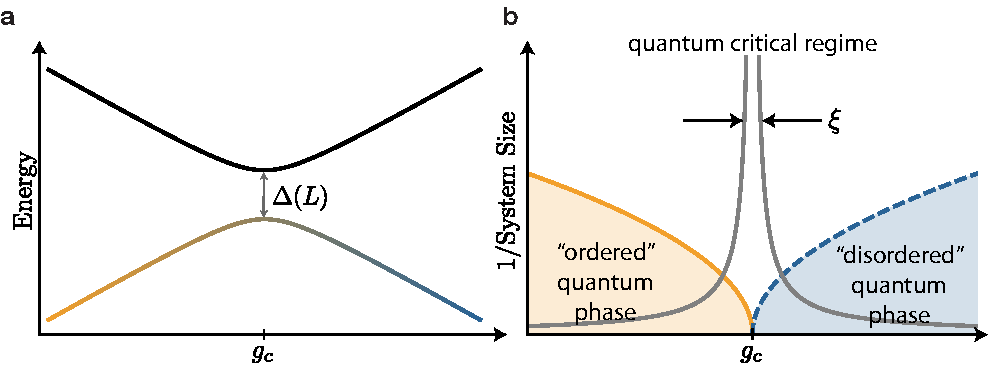
\includegraphics[width=\columnwidth]{figures/ch3/qpt_2.pdf} 
		\caption{\textbf{Equilibrium quantum phase transition. a)} The canonical schematic for a quantum phase transition occurring at $T=0$ for the ground state as a function of a tuning parameter $g$. The avoided crossing shown between the ground state and the excited state in this diagram are separated by the coupling between the two terms in the Hamiltonian:  $H_o$ and $H_1$. Each dominating character of the ground state in their respective regimes. The color of the ground state denotes whether it lies in the ``ordered" or ``disordered" phase. \textbf{b)}  The canonical phase diagram associated for a quantum phase transition has an ``ordered" and a ``disordered" phase that cross at a critical point $g_c$ when $T=0$. The left diagram, \textbf{a}, is just plot of the eigenstates along the $T=0$ cross section of this diagram. As the temperature is increased, more eigenstates in the system become incoherently populated and conceptually the quantum fluctuations, $\hbar \omega_c$, that attempt to order the system compete with the thermal fluctuations $k_b T$ that drive the system towards a disordered phase.  The closing gap near the critical point extends this classically disordered phase downward into the critical ``fan" shape associated with critical behavior and quantum phase transitions. A similar diagram can be made for the Temperature rather than inverse system size.}
		\label{fig:eq_qpt}	
\end{figure}

To probe all ground-state phase transitions, a system is typically prepared in one phase at equilibrium, then a parameter in the Hamiltonian, e.g. $\lambda$, has to be swept as a function of time through the transition point. These are also known as equilibrium phase transitions since the assumption is that this parameter is swept adiabatically. Since the Hamiltonian will not be time-independent during this sweep, the approximate requirement for adiabaticity is given by the Landau-Zener problem that the change in the energy due to the sweep of a parameter $(d\lambda /dt)\times(dE/d \lambda) < g$ where  $(d\lambda /dt)\times(dE/d \lambda)$ is the change in the energy as a function of time and $g$ is the coupling between the ground and excited states. Experimentally, any ramp will be finite in time, and any finite ramp time will always inject a finite amount of entropy into the system during the sweep. Additionally, even if these systems are prepared at $T\approx 0$, the degree to which this sweep is not adiabatic will result in non-equilibrium dynamics. The presence of these non-equilibrium dynamics are characteristic of the energy gap in the system defined by parameter $\lambda(t)$ when this adiabatic criterion breaks down due to the finite ramp time. This is additionally linked to the correlation length in the system which is dependent to the energy gap in the system and therefore defines the average size of domain size in a system \cite{Sachdev2011}. The relationship between this domain size, correlation length, and dynamics is known by the Kibble-Zurek mechanism \cite{Polkovnikov2005,Zurek2005} and have recently been seen experimentally\cite{Keesling2019}. 


\subsection{A non-equilibrium phase transition}

The thermal-to-MBL eigenstate phase transition is also known as an out-of-equilibrium phase transition.\footnote{This term additionally covers another class of ``dynamical phase transitions" that are qualitatively different from the thermalizing to MBL transition discussed here.}  Since it is not physically possible, while remaining in thermodynamic equilibrium, to populate a single highly excited eigenstate, the quantum quench performed in the experiment will populate many excited eigenstates which will lead to dynamics. However, an important point is that the many-body gaps between eigenstates are related to the properties of the eigenstates themselves and therefore the observed unitary dynamics probe the inherent characteristics of the eigenstates\cite{Huse2013,Nandkishore2015,Alet2018,Abanin2018}.


\begin{figure}[t!]
		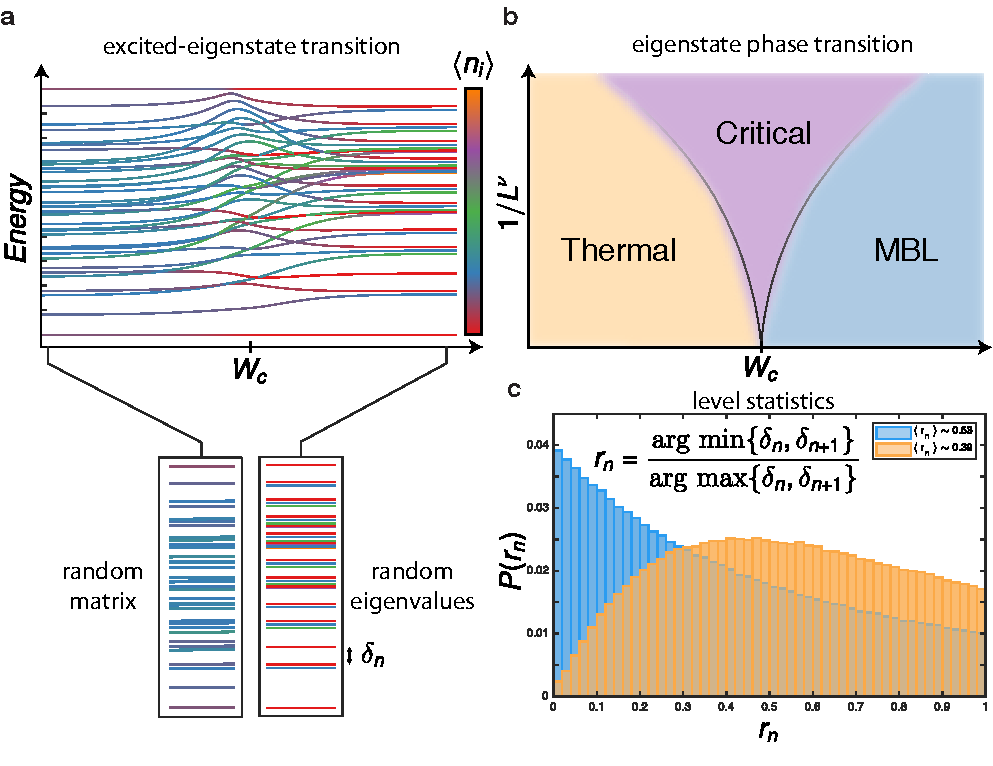
\includegraphics[width=\columnwidth]{figures/ch6/excited_eig_qpt.pdf} 
		\caption{\textbf{Excited eigenstate phase transition and spectral statistics. a)}  The entire spectrum (normalized in bandwidth) is plotted for a small, disordered Bose-Hubbard chain as a function of disorder strength $W$. The color of the eigenstates denote the local particle number on a single-site. Not only do we see a large number of crossings near the critical point, but the color of the eigenstates, which was very uniform for low disorder $(W<W_c)$, changes dramatically as it cross the transition $(W>W_c)$. By zooming into the spectrum on either side we can see the differences in gaps: on the low-disorder side there are level-repelled eigenstates that are characteristic of the eigenvalues of a random matrix and ergodic eigenstates, and on the high-disordered side we see gaps that change dramatically across the spectrum that is characteristic of random eigenvalues and non-ergodic eigenstates. \textbf{b)} The association of these characteristic gaps and local parameters expressed in \textbf{a} are associated with the generic behavior attributed to the excited eigenstates in the thermalized and many-body-locazlized phases. \textbf{c)} The common metric used to differentiate these two phases from their spectrum is by computing the level statistics ratio $r_n$. The histogram of values are plotted for a random matrix (orange, thermalizing regime) and randomly selected eigenvalues (blue, localized regime).}
		\label{fig:ex_eig_qpt}	
\end{figure}

In the thermalizing case (\S \ref{sec:ch4}), the ergodic nature of the eigenstates of the system imply that most relatively local properties change smoothly across the eigenstates as a function of energy. This can be intuited from the fact that by the property of being ergodic, small perturbations applied to any eigenstate will hybridize energetically nearby eigenstates. This property additionally leads to level repulsion between eigenstates and applies generically across the majority of the spectrum\cite{DAlessio2016}. \footnote{This level repulsion is nothing other than avoided level crossing in a two-level system when they are generically coupled by some parameter. For these thermalizing systems this applies generically between almost any two eigenstates since they are constructed out a nearly ergodic superposition of states that are constrained only by global, thermodynamic quantities.} It is precisely the non-ergodic character of a many-body-localized eigenstate that prevents a generic perturbation from coupling nearby energy eigenstates. Consequently, or simultaneously, this means that eigenstates also can change drastically in their local character from eigenstate to eigenstate and do not exhibit level repulsion. This internal character of these two phases is inherently related to their relative gaps in the system and hence their dynamics\cite{Huse2013}. A convenient metric, known as the level statistics ratio, captures the existence of this level repulsion and characterizes the transition of eigenstates from ergodic to non-ergodic:

\begin{equation}
\label{eqn:levelStat}
r_n \equiv \frac{\text{min}\{\Delta_n,\Delta_{n+1}\}}{\text{max}\{\Delta_n,\Delta_{n+1}\}}
\end{equation}

where $\Delta_n = E_n - E_{n-1}$ is the energy difference between neighboring eigenstates indexed  by $n$ in order of increasing energy. In the regime where the states are ergodic, the eigenenergies match those of the eigenvalues from a random matrix and the eigenstate average, $\langle r \rangle$ takes on the Wigner-Dyson value $\langle r \rangle \approx 0.53$. In the many-body localized regime the eigenvalues look as though sampled from a random distribution and are then characterized by the Poisson value $\langle r \rangle \approx 0.39$. The transition of a system's level statistics ratio is typically the way theory identifies these two regimes, however we will look at the resultant dynamic behavior of the system that is inherently linked to the structure of the eigenstates that are captured by this statistic (Fig.~\ref{fig:ex_eig_qpt}). 

Since this metric requires access to all the eigenstates and their relative gaps, it is mostly used as a theoretical tool\cite{Huse2013,Nandkishore2015}. Although, recently in a small qubit system the excitation spectrum was probed such that the spectrum could be reconstructed \cite{Roushan2017}. Lastly, as it is the gaps in the many-body spectrum that give rise to all observable dynamics, this change in eigenstate characteristics will be observable in the the dynamics of the system.

\subsection{Observing non-equilibrium critical dynamics}

Qualitatively, we can see the overlap of several characteristic traits between equilibrium quantum phase transitions and the thermal-to-MBL transition. In both cases, for some parameter regime, there exists a phase that is described by a local observable (order parameter or localization of initial state) and the eigenstates of both the ground state phases and excited states in MBL follow an area-law in entanglement entropy. However, several other characteristics seem difficult to relate, such as the notion of a diverging correlation length at the critical point in equilibrium transitions since eigenstates change from an area-law in the MBL phase to a volume-law in the thermal phase -- where correlations are scrambled among all constituents and therefore extended. Some of these comparisons are schematically shown in Fig.~\ref{fig:ex_eig_qpt} and Fig.~\ref{fig:eq_qpt}. 

Conceptually, though, the mechanisms may be similar in how the eigenstates change: phase transitions are driven by collective fluctuations of a system's constituents that emerge at a critical point \cite{Tauber2017,Sachdev2011,Landau1937}. We will probe the critical behavior of this non-equilibrium phase transition by observing the correlation dynamics that emerge at intermediate disorder near the critical point. By comparing multiple system sizes at fixed evolution time, we can probe which local behavior is critically dependent upon the system size and how the emergent correlation dynamics lead to this critical behavior.

We will again focus on the interacting Aubry-Andr\'e model\cite{Aubry1980}: 

\begin{equation}
\label{eqn:AAM}
H = -  J \sum_{\langle i,j \rangle}  \left ( \hat{a}_i^\dagger \hat{a}_j + \hat{a}_j^\dagger \hat{a}_i  \right ) + \frac{U}{2} \sum_{i} \hat{n}_i (\hat{n}_i - 1 ) + W \sum_i h_i \hat{n}_i
\end{equation}

where, $h_i = \cos (2 \pi \beta x_i + \phi)$ and with a spatial frequency of $\beta \approx 1.618$ sites${^{-1}}$ as an approximation of the golden ratio ($\beta_{GR} = \frac{\sqrt{5}+1}{2}$). We will follow the same quench protocol shown in the previous chapter \S \ref{sec:ch5} and pictorially shown in Fig.~\ref{fig:ch5fig2}. All experiments will use a unity-filling Mott insulator for the initial state for a system size of $L=8$ or $L=12$.

\section{Localization and transport}
\label{sec:AALoc}

We will first characterize the system's dynamical behavior by studying its transport properties at different disorder strengths. This will be similar to asking how local perturbations explore the remainder of the system and should characterize the thermalizing regime. Since the initial state has exactly one atom per site, the system starts with zero density correlations at all length scales. However, during the Hamiltonian evolution, the tunneling dynamics build up anti-correlated density fluctuations between coupled sites of increasing distance. Motivated by this picture, we quantify the particle dynamics by defining the transport distance:

\begin{equation}
\label{eqn:deltax}
\Delta x = 2 \sum_d d \times \langle G^{(2)}_c (i,i+d) \rangle
\end{equation}

as the first moment of the simultaneously disorder and site-$i$ averaged two-point density correlations, $G^{(2)}_c(i,i+d) = \langle \hat{n}_i \hat{n}_{i+d} \rangle - \langle \hat{n}_i \rangle \langle \hat{n}_{i+d} \rangle$. This two-point density correlation function correctly maps out the effective probability distribution of a single-particle in the non-interacting limit of the Aubry-Andr\'e model. Additionally, by calculating the first moment of the distribution we do not assume a particular functional form for the localization of particles. However, it is useful to compare to the analytical results for the non-interacting case to see how such a metric converges to the localization length. 

In the large detuning limit, one can find that all states are localized by the large site-to-site detuning quantified by on-site disorder W:

\[
\psi \sim \frac{1}{\mathcal{N}} \sum_d (2 J/W)^d = \frac{1}{\mathcal{N}} \sum_d e^{-d/\xi}
\]

where $\frac{1}{\xi}=\log{(2 J/W)}$. Analytically, it was shown by Aubry and Andr\'e that $\frac{1}{\xi}=\log{(\lambda/2)}$ where $\lambda = W/J$\cite{Aubry1980}. We then extract the first moment of this localized function:
%\[
%P(x_i) = \frac{1}{\mathcal{N}} \sum_i e^{-x_i / \xi}
%\]

\[
\langle x \rangle = \frac{1}{\mathcal{N}} \sum_i x_i~e^{-x_i /\xi}= - \frac{\partial}{\partial (1/\xi)}  \frac{1}{\mathcal{N}} \sum_i e^{-x_i /\xi} = \frac{1}{e^{1/\xi} - 1} 
\]

By expanding the exponential of this result we see that the localization length and the first moment, $\langle x \rangle$ converge  in the large localization length limit. 

\[
1+\frac{1}{\langle x \rangle} = e^{1/\xi} \approx 1 + \frac{1}{\xi} + \mathcal{O}(2) ...
\]


It also allows us to compare the expected first moment a a given disorder strength in the non-interacting limit:
\[
\langle x \rangle = \frac{1}{w/2 - 1}
\]

However, this last dependence on the disorder strength will not prove quantitatively precise in our case since the localization point significantly changes in the case of an interacting system and it is not known if the scaling behavior should be the same in the interacting system. Qualitatively though, it provides a usable metric that is model independent and maps onto the correct quantity when the system is exponentially localized. There is an additional complication in the interacting case: when comparing this value across different disorder strengths, the injected energy by the quench changes the number of participating particles.\footnote{Since the particles harbor repulsive interactions, high on-site occupancy costs more injected energy. Therefore by injecting a finite amount of energy only favors lower on-site occupations and effectively appears as though only a fraction of the particles are participating in the delocalization.} We normalize this effect by adding an additional normalization constant to create the normalized first moment $\Delta \tilde{x}$:

\begin{equation}
\label{eqn:normg2}
\Delta \tilde{x} = \frac{2 L}{L-1} \left (\frac{\sum_d G^{(2)}_c(d)~d }{\sum_d G^{(2)}_c(d)} -1 \right )
\end{equation}

This function is normalized such that in the thermalizing regime, where particles are completely delocalized, that the normalized first moment $\Delta \tilde{x}$ is equal to the system size $L$. We measure this quantity for several disorder strengths after long evolution times, $t/\tau \approx 100$, such that the system's dynamics should have saturated for our system sizes. We show this in Fig.~\ref{fig:intCorrLen} both experimentally and numerically to demonstrate how these quantities differ for the interacting and non-interacting regimes. Note that the point where the single-particle localization transition should occur is $W_c = 2 J$ and is approximately where the single particle normalized transport distance decreases from the system size. In the deep disorder regime, the transport distance is similar for both system sizes. Additionally, the agreement of the theoretically predicted transport distance for an interacting and non-interacting system indicates the negligible role of interactions in transport in the strongly localized regime. Although we expect this might be true asymptotically, it could be the closeness of convergence at this disorder depth is finite-time limited.


\begin{figure}
\floatbox[{\capbeside\thisfloatsetup{capbesideposition={left,top},capbesidewidth=2.5 in}}]{figure}[\FBwidth]
{\caption{\textbf{Transport distance: interacting and non-interacting.} The first moment is plotted as a function of disorder strength $W$ for both the interacting (solid, points) and the non-interacting (dashed) cases for both the $8,12$-site systems. The first moment remains close to the system size till $W\approx5J$ when it begins to localize for the interacting case. The first moment remains close to the system size till $W\approx2J$ when it begins to localize for non-interacting. The solid lines are computed by exact numerics. The error bars are the s.e.m.}\label{fig:intCorrLen}}
{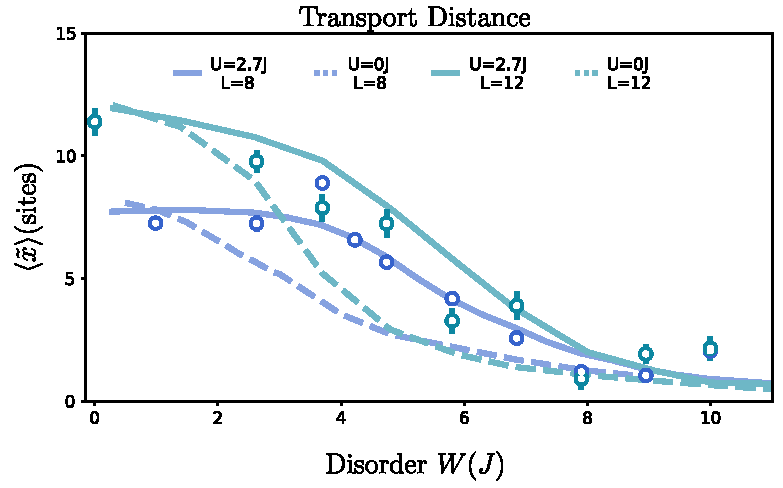
\includegraphics[width=3.5 in]{figures/ch6/XiLenComp.pdf}} 
\end{figure}


\section{Critical transport behavior}

Now that we have an idea of where the system changes phases from delocalized to localized, we can probe the inherent dynamics involved at the transition point of such a non-equilibrium phase transition. We additionally only evaluate these critical dynamics for the $L=8$ system size since we can only locate the finite-size critical regimes by comparison to larger system size. This will be further clarified below.


\subsection{Anomalous diffusive transport}

At low disorder, we observe that anti-correlations rapidly build up and saturate with a time scale of $t/\tau \approx L/2$. Note that this is the approximate time it takes for a ballistic density excitation to travel across the entire system size $L$ since the tunneling time $\tau = 1/(2\pi J)$  where $J$ is defined in the hopping rate of the field of the quantum many-body wave function. With increasing disorder, we observe a slowdown of particle transport that is consistent with a power-law growth $\Delta x \sim t^\alpha$ (Fig.~\ref{fig:crTherm}) \cite{Agarwal2015,Setiawan2017,Zhang2018,Garrison2018}. We extract the power-law exponent $\alpha$ from the data points after the initial transient dynamics cease ($L/2 < t/\tau \leq 100$) (Fig.~\ref{fig:crTherm} inset). We find that this exponent $\alpha$ is reduced by successively higher disorder strengths such that it is only anomalously diffusive in the intermediate disorder regimes and demonstrates the suppression of transport in the MBL regime at high disorders.\footnote{Note that the thermal regime is expected to eventually become $\alpha=0.5$ in the infinite size limit. However, finite size effects limit both our experiment and numerical simulations which attempt to probe this regime.\cite{Agarwal2015}} We cannot experimentally verify the functional form of the transport behavior, but can find a very suggestive relationship numerically which is shown in Appendix: \ref{appendix:Ch6Cal}. 

\begin{figure}[t!]
		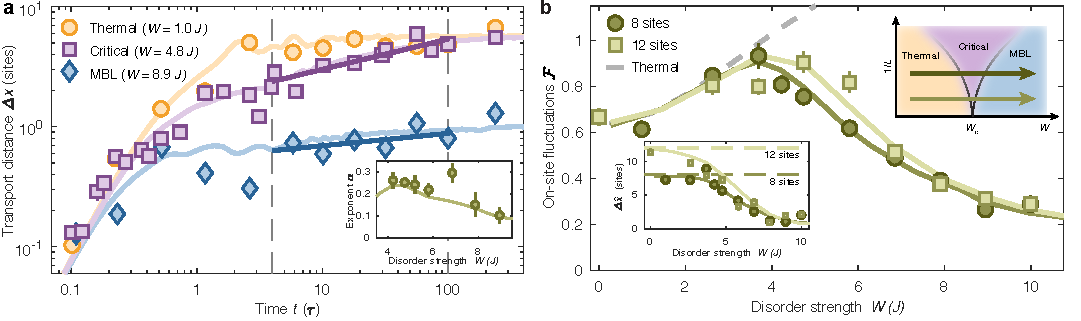
\includegraphics[width=\columnwidth]{figures/ch6/fig2a.pdf} 
		\caption{\textbf{Critical Thermalization. a)}   Particle transport slows down at intermediate disorder, consistent with a power-law evolution with exponent $\alpha<0.5$, demonstrating subdiffusive dynamics (inset). These data were taken on an eight-site system. \textbf{b)} The critical nature of these dynamics is determined from the behavior of on-site density fluctuations $\mathcal{F}$ and transport distance $\Delta \tilde{x}$ (lower left inset) for both considered system sizes. The thermal regime is determined by the agreement of the measured $\mathcal{F}$ with the prediction from a thermal ensemble (dashed grey). The system-size dependence at intermediate disorder is consistent with the reduced size of a quantum critical cone (upper right inset). These data were measured for both an eight-site and twelve-site system. The solid lines denote the prediction of exact numeric time calculations without any free parameters. The errorbars are the s.e.m.}
		\label{fig:crTherm}	
\end{figure}

\subsection{Critical thermalization}

In order to identify the anomalous diffusion as a signature of quantum critical behavior, we measure the system-size dependence of two observables in the long-time limit (t=100 $\tau$): the on-site number fluctuations $\mathcal{F} \equiv G_c^{(2)} (d=0) $ as a probe of local thermalization and the corresponding transport distance $\Delta \tilde{x}$ as a measure of localization (Fig.~\ref{fig:crTherm}). At low disorder, the fluctuations agree with those predicted by a thermal ensemble and particles are completely delocalized for both system sizes ($L=8,12$). This demonstrates that local quantum thermalization in our system is system-size independent at low disorder and identifies this disorder regime as the thermal phase. At strong disorder, the physics is governed by the formation of an intrinsic length scale, namely the localization length $\xi \sim \Delta \tilde{x}$ \cite{Choi2016,Lukin2019}(\S \ref{sec:AALoc}). We observe system-size independent, sub-thermal fluctuations that measure the onset of an intrinsic length scale. This identifies the strong disorder regime as the localized phase. However, at intermediate disorder, our data are consistent with a system-size dependence for both observables. This simultaneously demonstrates the absence of an intrinsic length scale and the presence of finite-size-limited fluctuations and hence finite-size-limited thermalization, therefore identifying the presence of a critically thermalizing regime. These measurements of system-size dependent, enhanced thermalization can be visualized as two horizontal cuts in a finite size phase diagram. The observed finite-size dependence is consistent with the physics associated with a critically thermalizing intermediate phase and a shrinking quantum critical cone (Fig.~\ref{fig:crTherm}).\footnote{This, however, only demonstrates that the $L$=$8$ system is critically sub-thermal for the intermediate disorder regime and continues to thermalize in the presence of a larger system. Without having any other measurement, a strict statement about the $L=12$ system being critical cannot be made.}

\subsection{Fluctuations scaling}

One complication with scaling the thermal predictions to larger system sizes is that the classical ensemble prediction still requires knowing all the energy eigenstates in the Hamiltonian. However, there is an analytical approach to finding the particle-number fluctuations per particle for a given sub-system at infinite temperature that will help provide some intuition:

\begin{equation}
\label{eqn:FNL}
\mathcal{F}(l,N)_L/N = \left ( \frac{\left ( L-l \right ) l }{L^2} \right ) \left ( \frac{ 1+N/L }{ 1+1/L } \right )
\end{equation}

where $l$ is the sub-system size, $L$ is the total system size, and $N$ is the total particle number (see Appendix: \ref{appendix:Ch6Cal} for derivation). Note that in the limit that $N\rightarrow 1$ this reduces to the fluctuations per particle given by a Bernoulli distribution:

\[
\mathcal{F}(l,N)_L/N = \left ( \frac{\left ( L-l \right ) l }{L^2} \right )
\]

 The factor of $N/L$ (typically denoted as the filling of the system $\nu$) arises from indistinguishability of the bosons and their enhanced likelihood to occupy the same quantum-mechanical state (known as bosonic enhancement).  However, since our system is always at some finite energy density, the number of excitations in the system that then participate in these fluctuations becomes limited to some effective number $N\rightarrow N_{eff}$. We do not know of any literature that defines what the correct energetic suppression of this $N$ should be. This scaling of such subsystem fluctuations also contain the physics of the localization length in the system and can additionally be used to probe the transition point. In the thermal regime, the particles are delocalized and so the fluctuations are qualitatively similar to the expression above (\ref{eqn:FNL}) up to an overall scaling. Therefore, by evaluating the half-size subsystem fluctuations we expect the fluctuations to scale with the volume of the total system ($\mathcal{F}(l=L/2,N=L)_L \sim L$). Conversely, as the particles become localized the system forms an intrinsic length scale $\xi$ that particles can delocalize over that does not scale with the total system size. This intrinsic length scale would give rise to a strict area law ($\mathcal{F}(l=L/2,N=L)_L \sim const.$)\cite{Singh2016}. We explore the scaling behavior of these half-system size fluctuations for three system sizes: $\{ L=6, L=8, L=12\}$ in Fig.~\ref{fig:bpF}. A possible relationship between the scaling behavior and the localization length $\xi$ is discussed in Appendix: \ref{appendix:Ch6Cal}.

\begin{figure}[t!]
\floatbox[{\capbeside\thisfloatsetup{capbesideposition={right,top},capbesidewidth=2.6 in}}]{figure}[\FBwidth]
{\caption{\textbf{Scaling of bipartite fluctuations.} The scaling of half-system size, bipartite fluctuations $\left (\mathcal{F}_L(l=L/2,t=100\tau \right)$ are plotted here for data taken at three system sizes: $\{ L=6, L=8, L=12\}$. These data are always measured after long evolution times $(t=100\tau)$ and then fit with a power law as a function of half-system size $L$. The fitted exponents are then plotted in the inset. The solid lines denote the fitted values from a power law. The error bars are the s.e.m.} \label{fig:bpF}}
{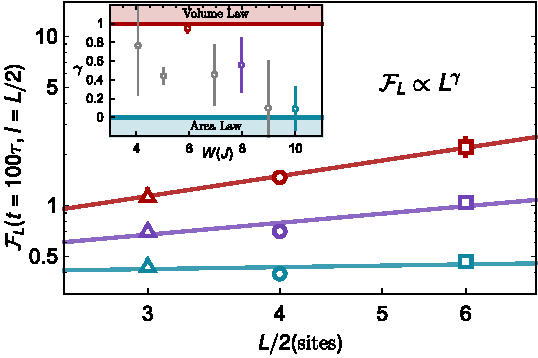
\includegraphics[width=3.6 in]{figures/ch6/combo_fluc.pdf} } 
\end{figure}

\section{Correlation Structure}

In order to reveal the microscopic origin of this anomalous transport, we now investigate the site-resolved structure of correlations in the many-body state (Fig.~\ref{fig:corrStructure}\textbf{a}). We first study how much each lattice site contributes to the transport by considering the site-resolved two-point correlations in the long-time limit ($t=100 \tau$). In the thermal regime, we find similar correlations between all lattice sites, which correspond to uniformly delocalized atoms. In contrast, density correlations are restricted to nearby sites in the MBL regime due to localization. Intriguingly, we observe a sparse structure of correlations at intermediate disorder, which involves only specific distances between lattice sites, yet spans the entire system.

\begin{figure}[t!]
\floatbox[{\capbeside\thisfloatsetup{capbesideposition={right,top},capbesidewidth=3 in}}]{figure}[\FBwidth]
{\caption{\textbf{$G^{(2)}(d)$ Structure. a)} The measured site-dependent two-point correlations $G^{(2)}_c(i,j)$  differ for the three disorder regimes. In the quantum critical regime, correlations preferably form at specific distances, showing a network-like structure. This contrasts with homogeneous correlations in the thermal regime and nearest neighbor correlations in the MBL regime. \textbf{b)} The structure of the correlation network is revealed by the averaged correlation function $G^{(2)}_c(d)=\langle G^{(2)}_c(i,i+d)\rangle_i$. Its similarity to the autocorrelation $A(d) = \langle h_i h_{i+d}\rangle_i$ of the quasi-periodic potential (solid grey) indicates interaction-induced tunneling processes that are enhanced when the interaction energy compensates for the chemical potential difference. \textbf{c)} We quantify the similarity by the overlap $\mathcal{B}=\sum_d G^{(2)}_c(d) A(d)$, which is maximal in the quantum critical regime. The sign of the overlap would be opposite for non-interacting particles (dashed line), which favors tunneling between sites with similar potential energies. The solid lines in \textbf{b,c} denote the prediction of exact diagonalization calculations without any free parameters. The error bars are the s.e.m.} \label{fig:corrStructure}}
{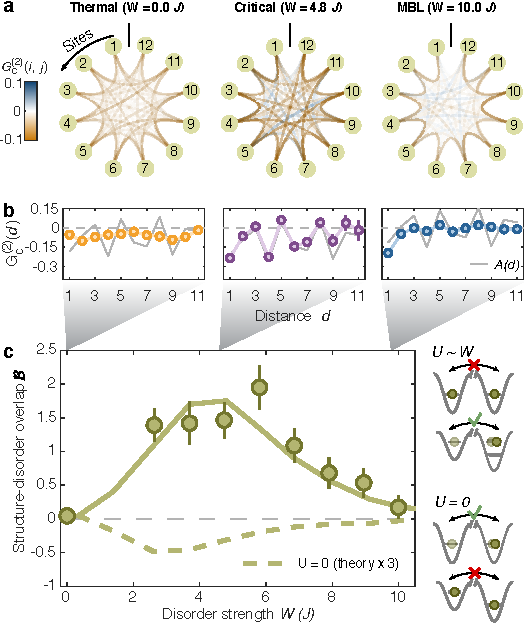
\includegraphics[width=3 in]{figures/ch6/fig3.pdf} } 
\end{figure}

The sparse resonant structure is expected to be linked to the applied quasi-periodic potential. The average energy offsets of distances $d$ apart in the system are correlated by this potential. The correlation is then inherited by the system's fluctuations when the interaction energy $U$ compensates for these correlated offsets. To investigate this structure, we compare the two-point density correlations with the autocorrelation function, $A(d) = \langle h_i h_{i+d} \rangle_i$, of the quasi-periodic potential. Indeed, we find that the site-averaged density correlations $G^{(2)}_c(d) = \langle G^{(2)} (i,i+d) \rangle_i$ inherit their spatial structure from $A(d)$ (Fig.~\ref{fig:corrStructure}\textbf{b}). We quantify this contribution by taking the overlap of these two-point correlation functions, $\mathcal{B} = \sum_d \langle G^{(2)} (i,i+d) \rangle_i A(d)$. We find find that this contribution is maximal in the critical regime but is strongly reduced in both the thermal and MBL regimes (Fig.~\ref{fig:corrStructure}\textbf{c}). These observations contrast with the behavior of a non-interacting system, where the sign of the structure is opposite since resonant tunneling is favored for zero potential energy difference between sites (Fig.~\ref{fig:corrStructure}\textbf{c}). These results illustrate microscopically how the interplay of strong interactions and disorder can lead to anomalous diffusion. However, this picture of effective single-particle hopping that couples distance sites neglects the potential many-body nature of these systems and the emergence of collective fluctuations between many particles over long distances.

\section{High-order Correlations}

We investigate the contribution of multi-particle fluctuations to the thermalization in the critical regime to probe the presence of enhanced quantum fluctuations when the system changes phases. For this study, we employ the $n$-point connected density-correlation functions \cite{Liu2016,Schweigler2017,Hodgman2017,Preiss2019}:

\begin{equation}
\label{eqn:gcon}
G^{(n)}_c(\textbf{x}) = G^{(n)}_{tot} (\textbf{x}) - G^{(n)}_{dis} (\textbf{x})
\end{equation}

which acts on lattice site positions $\textbf{x} = ( x_1, ..., x_n)$. The disconnected part of this function, $G^{(n)}_{dis}$ is fully determined by all lower-order correlation functions, and therefore does not contain new information at order $n$. By removing these disconnected contributions from the total measured correlation function, $G^{(n)}_{tot} = \langle \prod_i^n \hat{O}_i \rangle$, we isolate all $n$-order correlations that are independent of lower-order process (\S Appendix: \ref{appendix:Ch6Cal}). This approach gives a direct handle on the level of complexity of the underlying correlation structure of the many-body wave function and characterizes its entanglement via its non-separability into subsystems of size $<~n$. We quantify the relevance of order $n$ processes by computing the mean absolute value of all correlations arising from both contiguous and non-contiguous $n$ sites in the system (Fig.~\ref{fig:highOrder}). This is similar to looking at the width of the distribution of correlations at a given order since the average correlation value converges to zero. This is conceptually similar to investigating the network structure  at higher disorders since this width will disappear in the thermal and localized phases as all correlations will be equivalent or only local, respectively. The distributions of the correlations for high-orders for various disorder strengths and sampling sizes are plotted in \S Appendix: \ref{appendix:Ch6Cal}. 

\begin{figure}[t!]
		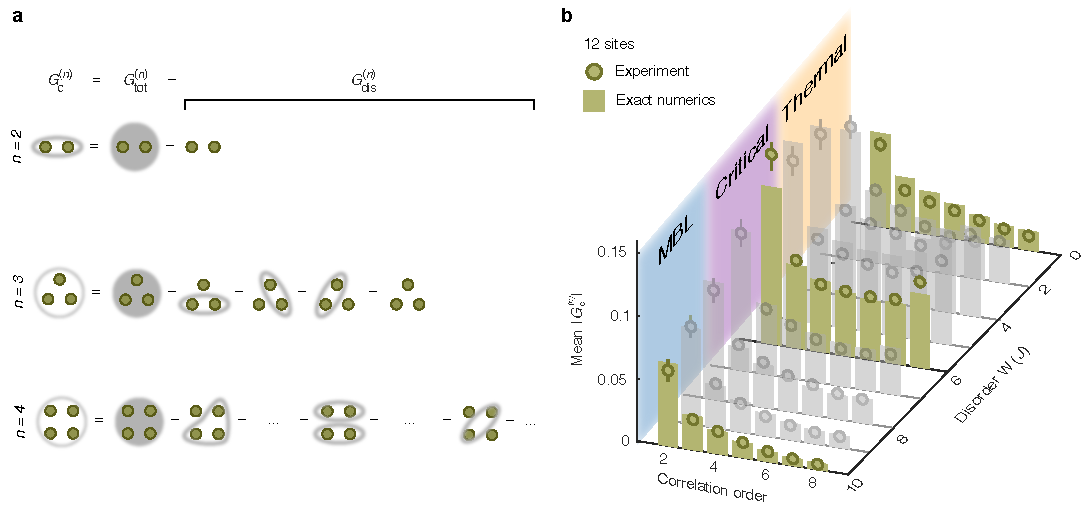
\includegraphics[width=\columnwidth]{figures/ch6/fig2b.pdf} 
		\caption{\textbf{Higher Order Connected Correlations. a)}  We obtain the genuine many-body processes of order $n$ from connected correlations $G_c^{(n)}$ by subtracting all lower order contributions $G_\text{dis}^{(n)}$ from the total correlation function $G_\text{tot}^{(n)}$. \textbf{b)} In the quantum critical regime, we find enhanced collective fluctuations at all measured orders by computing the mean absolute value of $G_\text{c}^{(n)}$ for different disorder strengths. These data were measured on a twelve-site system.The bars denote the prediction of exact numeric time calculations without any free parameters. The error bars are the s.e.m.}
		\label{fig:highOrder}	
\end{figure}

We find that in the thermal and the many-body-localized regimes, the system becomes successively less correlated at higher order. The behavior in the quantum critical regime is strikingly different: we observe that the system is strongly correlated at all measured orders. There is an additional interpretation to the presence of correlations at high order that relates to the length scale of entanglement in the system. Since all high-order correlations in this system inherently involve $n$ unique sites, it is also implying that there is non-negligible correlations across $n$ sites in the system and can be thought of as an increasing length scale of correlations in this critical regime. Similar behavior has been seen in theory when performing a cluster analysis of entanglement among spins \cite{Herviou2019} and is reminiscent of the canonical phase transition behavior expected for equilibrium phase transitions\cite{Amico2008, Osterloh2002,Osborne2002}.

In order to further investigate the system's many-body structure, we examine the site-resolved contributions of the three-point correlations. Since all non-zero contributions to the three-point correlations involve correlated hopping of at least two particles, they are a signature for multi-particle entanglement\cite{Schweigler2017}.  In the quantum critical regime, we find that these correlations span the entire system and are highly structured, taking on both positive and negative values (Fig.~\ref{fig:g3microscopy}). In contrast to the pattern in the second-order correlation function, this third-order structure is not directly recognizable as the quasi-periodic correlation functions. In fact, the quasi-periodic correlation function is exactly zero at third-order. In order to gain further insight into the structure, we analyze the contributions of all possible particle configurations that contribute to non-zero connected correlations in Fig.~\ref{fig:g3microscopy}. In particular, for $G^{(3)}_c(d_1=3,d_2=1)$, which is positive, we see that the dominant contributions comes from a particular process that favors multiple atoms hopping to the same site. In contrast, $G^{(3)}_c(d_1=3,d_2=2)$, which is negative, has a dominant process that favors all atoms leaving the three considered sites. While this provides some intuition for the emergent many-body resonances, the three-point correlations are, in fact, the result of a superposition of many correlated processes. These observations further demonstrate how the interactions between multiple atoms can compensate for the disorder via correlated tunneling of several atoms. In this way we can see the additional role interactions play in the disordered system: they supply high-order many-body resonances that preserve transport where lower-order processes are energetically suppressed.

\begin{figure}[t!]
		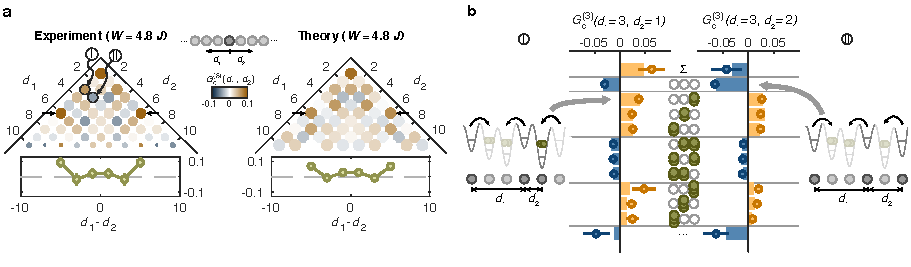
\includegraphics[width=\columnwidth]{figures/ch6/fig4.pdf} 
		\caption{\textbf{Microscopy of $G^{(3)}_c(d_1,d_2)$. a)}  The connected correlation function, $G^{(3)}_c(d_1,d_2)$, for three lattice sites spaced by distances $d_1$ and $d_2$ in the quantum critical regime $(W=4.8J)$, showing the strongly interacting nature of the state. We find that the three-point correlations show a characteristic structure that is governed by the contribution of the number states on the considered sites. The arrows indicate the cut in $d_1,d_2$ space plotted below. \textbf{b)} To exemplify the relevant processes of order n=3, we show the contributions of the number states on lattice sites at distance $d_1=3$, $d_2=1$ (left) and $d_1=3$, $d_2=2$ (right). While there is a wide distribution of contributing configurations, the relative dominance of a particular process provides the overall structure in \textbf{a}. The illustration of atoms undergoing a highly correlated hopping process in the lattice describe how such correlations can contribute to either positive or negative correlations among the three considered sites. The theory plot in \textbf{a} and bars in \textbf{b} are calculated from exact numeric time calculations without any free parameters. The inverse marker size in the experimental plot in \textbf{a}, and the error bars in both \textbf{a} and \textbf{b} denote the s.e.m. }
		\label{fig:g3microscopy}	
\end{figure}

\section{Discussion}

These results\cite{Rispoli2018} demonstrate how a many-body sparse resonant structure drives the quantum critical behavior at the MBL transition. The observed microscopic description is consistent with the theoretically suggested mechanism of a sparse \emph{backbone} of resonances that can act as a functional bath for the system that is critically sub-thermal \cite{Khemani2017, Grover2014, Potter2015}. However our results provide a new perspective on this description by mapping out the prevalence of higher-order process in the system that facilitate this critical thermalization.

Since we use a quasi-periodic localizing potential, our system has no rare regions and prevents other proposed thermalizing mechanisms from playing a role, such as rare Griffiths regions that act as local thermal baths. In that respect, we are able to isolate a class of thermalizing mechanisms and observe them in-situ as the dominant way that the system critically thermalizes at intermediate disorder. These results do not, however, rule out any other possible mechanism that may also lead to critical thermalization at intermediate disorder regimes. Further studies of larger system sizes and different localization potentials would better elucidate whether proposed mechanisms (e.g. quantum avalanches) would also lead to qualitatively similar behaviors \cite{Potter2015,Vosk2015,Zhang2018,Roeck2017,Luitz2017,Ponte2017}. This would additionally open up the possibility for studying the role of universality and whether there exist multiple classes for the thermal-to-MBL transition that depend upon the disorder type\cite{Khemani2017a}. 

A last comment to make is about what is considered a natural route of continued exploration, which would be to evaluate the same type of system at larger sizes. It is worth noting here that, at least for all known current experimental apparatuses, larger system sizes are not actually the limitation. The ability to evolve the quantum many-body system coherently for exponentially long time is the current limitation. The danger being that, in most cases, coupling to the external environment will add an energy reservoir attached to every site in the system that will always lead the system to an infinite temperature state given enough time. One of the crucial steps in the reported results from this thesis being that we are able to verifiably provide a bound on how coherent the system is (\S \ref{sec:ch5dec}). 






